\chapter{ATLOD: A Terrain Level of Detail (Renderer)}
This chapter describes \textit{ATLOD} (short for \textbf{A} \textbf{T}errain \textbf{L}evel \textbf{o}f \textbf{D}etail (Renderer)), the demo terrain rendering application.

\section{Preliminaries}
\subsection{Used Technologies}
ATLOD is written in C++17 and OpenGL 4.2.
For compiling build files, CMake (minimum version 3.5) is used.
ATLOD uses the following third-party libraries:
\begin{itemize}
  \item GLM: The \textit{OpenGL Mathematics (GLM)} library provides functionality for the mathematics of graphics programming, such as classes for vectors, matrices and perspective transformations.
  \item GLEW: The \textit{OpenGL Extension Wranger Library (GLEW)} is an extension loading library for OpenGL. 
  \item GLFW: \textit{GLFW} is a multi-platform library for desktop-based OpenGL applications, offering an API for managing windows, contexts and input handling.
  \item STB: STB is a collection of header-only libraries developed by Sean Barrett TODO cite. ATLOD uses \texttt{stb\_image.h} for loading images of heightmaps and textures.
\end{itemize}

ATLOD was developed with Qt Creator 9.6.1. The source code is hosted on GitHub on the repository AmarTabakovic/3d-terrain-with-lod
and is licensed under TODO.

\subsection{Chosen Algorithms}
The chosen algorithms and their reasons for implementing them are the following:
\paragraph{Naive Brute-force Algorithm} The naive brute-force algorithm consists of simply reading in all height values from the heightmap as vertices and rendering them directly to the screen.
The main reason for implementing the naive brute-force algorithm is to motivate the usage of terrain LOD algorithms by showing the difference in performance
compared to the optimized LOD approaches.

% TBD, depends on how far I come
\paragraph{GeoMipMapping} The main reason for implementing GeoMipMapping is its simplicity.

% \paragraph{Hoppe and Lossaso's Geometry Clipmaps} TODO
% \paragraph{Strugar's CDLOD} TODO

\section{Height and Texture Data}
\subsection{Data Sources}
\subsubsection{SwissTopo}

\subsubsection{SRTM}

\subsection{Supported Formats}
The following file formats are supported for loading heightmaps:
\begin{itemize}
  \item \texttt{.png} and \texttt{.jpg}: Heightmaps can be loaded as PNG and JPG images. This is implemented using \texttt{stb\_image.h}.
  \item \texttt{.asc}: Heightmaps as ASCII grids are supported. Digital elevation data from the Shuttle Radar Topography Mission (SRTM) is delivered in ASCII grid format.
  \item \texttt{.xyz}: the XYZ format is based on SwissTopo
\end{itemize}


\section{Basic Setup and Architecture}
\subsection{Overview}
TODO High-level class diagram

\subsection{Shaders}

\subsection{Camera}

\subsection{Heightmaps}

\subsection{Base Terrain}
Each terrain LOD algorithm is encapsulated in a class, which inherits from the base terrain class \texttt{Terrain}.
The base terrain is structured as shown in listing TODO.

\section{Naive Brute-force Algorithm}
The naive brute-force algorithm, which simply renders every vertex without any LOD considerations, is encapsulated in the class \texttt{NaiveRenderer}.

The method \texttt{loadBuffers()} loads the height data from the heightmap directly into a vertex buffer with the ID \texttt{terrainVBO} and the indices into an index (i.e. element) buffer named \texttt{terrainEBO}.
The indices are organized such that they can be rendered as triangle strips with \texttt{GL\_TRIANGLE\_STRIPS}.
Each row is separated using a special marker index named \texttt{RESTART}, which is set to the maximum possible \texttt{GLuint} value and is used for the \texttt{GL\_PRIMITIVE\_RESTART} mode,
allowing for the entire terrain to be rendered in a single \texttt{glDrawElements()} call. This draw call happens every frame in the 
method \texttt{render()}. Figure~\ref{fig:naive-triangles} shows the organization of indices for rendering the terrain as triangle strips.

\begin{figure}[H]
  \centering
  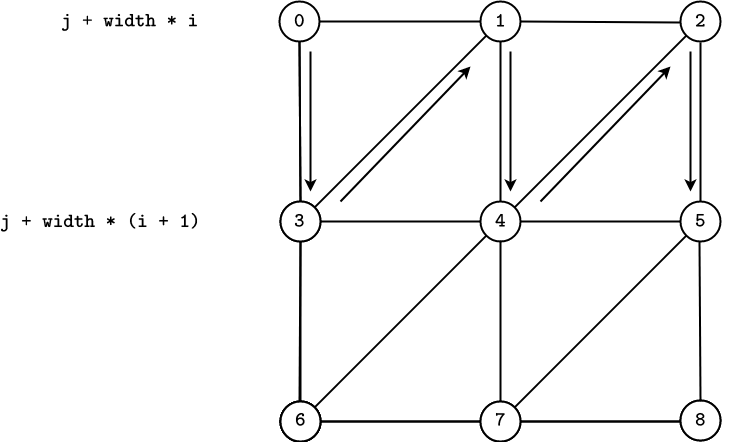
\includegraphics[width=0.9\textwidth]{atlod-naive-triangles}
  \caption{Example of a terrain layout for triangle strips. The looping index \texttt{i} goes from 0 to the terrain height and \texttt{j} from 0 to the terrain width. The final indices to be rendered are \texttt{0,3,1,4,2,5,RESTART,3,6,4,7,5,8,RESTART}.}\label{fig:naive-triangles}
\end{figure}

\section{GeoMipMapping}
ATLOD's GeoMipMapping implementation contains the basic GeoMipMapping features 
described in sections 1 and 2 in the original paper. 
The algorithm is encapsulated in the class \texttt{GeoMipMapping} and differs in certain aspects:
\begin{itemize}
  \item This GeoMipMapping implementation makes use of vertex and index buffers, which are more efficient than 
        rendering vertices in immediate mode. The organisation of vertices and indices is described in more detail in the subsection ``Vertex and Index Organisation''.
  \item The vertex omission for avoiding cracks is implemented somewhat differently from the original paper. 
        Instead of drawing triangle fans as shown in figure~\ref{fig:geomipmapping-crack-avoidance}, this implementation 
        uses the alternative approach shown in figure~\ref{fig:geomipmapping-crack-avoidance-alternative}.
\end{itemize}

\subsection{Data Structures}

\subsection{Vertex and Index Organisation}
Vertices are loaded into the vertex buffer in the method \texttt{loadBuffers()}. 

\begin{figure}[H]
  \centering
  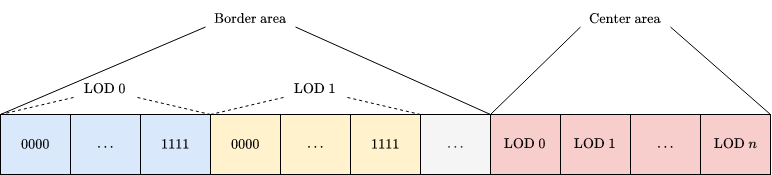
\includegraphics[width=1.0\textwidth]{atlod-geomipmapping-index-buffer.png}
  \caption{The index buffer organisation of a single block for the ATLOD's GeoMipMapping implementation. The variable $n$ is from the block size equation $2^n + 1$ and corresponds to the maximum LOD level.}\label{fig:atlod-geomipmapping-index-buffers}
\end{figure}

\subsection{Avoiding Cracks}

\begin{figure}[H]
  \centering
  \subfloat[\centering \texttt{0000}.]{{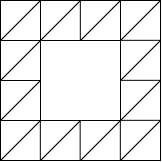
\includegraphics[width=0.17\textwidth]{atlod-geomipmapping-0000.png} }}
  \qquad
  \subfloat[\centering \texttt{0001}.]{{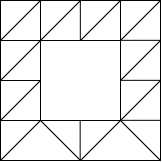
\includegraphics[width=0.17\textwidth]{atlod-geomipmapping-0001.png} }}
  \qquad
  \subfloat[\centering \texttt{0010}.]{{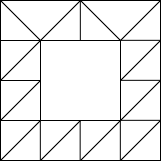
\includegraphics[width=0.17\textwidth]{atlod-geomipmapping-0010.png} }}
  \qquad
  \subfloat[\centering \texttt{0011}.]{{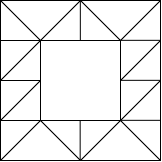
\includegraphics[width=0.17\textwidth]{atlod-geomipmapping-0011.png} }}

  \subfloat[\centering \texttt{0100}.]{{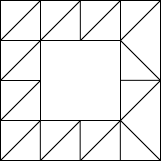
\includegraphics[width=0.17\textwidth]{atlod-geomipmapping-0100.png} }}
  \qquad
  \subfloat[\centering \texttt{0101}.]{{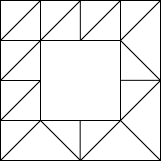
\includegraphics[width=0.17\textwidth]{atlod-geomipmapping-0101.png} }}
  \qquad
  \subfloat[\centering \texttt{0110}.]{{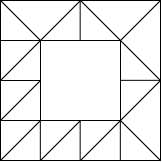
\includegraphics[width=0.17\textwidth]{atlod-geomipmapping-0110.png} }}
  \qquad
  \subfloat[\centering \texttt{0111}.]{{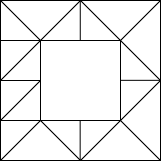
\includegraphics[width=0.17\textwidth]{atlod-geomipmapping-0111.png} }}

  \subfloat[\centering \texttt{1000}.]{{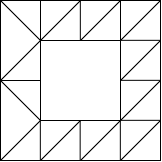
\includegraphics[width=0.17\textwidth]{atlod-geomipmapping-1000.png} }}
  \qquad
  \subfloat[\centering \texttt{1001}.]{{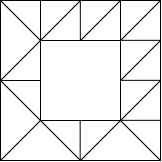
\includegraphics[width=0.17\textwidth]{atlod-geomipmapping-1001.png} }}
  \qquad
  \subfloat[\centering \texttt{1010}.]{{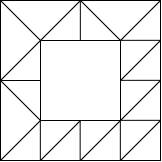
\includegraphics[width=0.17\textwidth]{atlod-geomipmapping-1010.png} }}
  \qquad
  \subfloat[\centering \texttt{1011}.]{{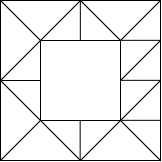
\includegraphics[width=0.17\textwidth]{atlod-geomipmapping-1011.png} }}

  \subfloat[\centering \texttt{1100}.]{{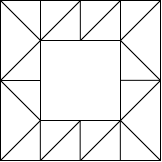
\includegraphics[width=0.17\textwidth]{atlod-geomipmapping-1100.png} }}
  \qquad
  \subfloat[\centering \texttt{1101}.]{{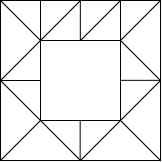
\includegraphics[width=0.17\textwidth]{atlod-geomipmapping-1101.png} }}
  \qquad
  \subfloat[\centering \texttt{1110}.]{{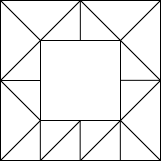
\includegraphics[width=0.17\textwidth]{atlod-geomipmapping-1110.png} }}
  \qquad
  \subfloat[\centering \texttt{1111}.]{{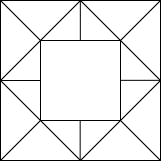
\includegraphics[width=0.17\textwidth]{atlod-geomipmapping-1111.png} }}
  \caption{Every possible border subblock configuration for a LOD 2 GeoMipMap of a $5 \times 5$ block. The bits (read from left to right) represent the left, right, top and bottom borders and are set to 1 if the bordering block on the corresponding side has a lower LOD, and 0 otherwise. The center subblocks have been omitted from the illustration.}\label{fig:atlod-geomipmapping-popping-avoidance}
\end{figure}
In order for this approach to work, the difference in LOD level between any two bordering blocks 
must be at most 1. 

\subsection{Rendering}
The method \texttt{render()} that is called each frame updates and renders the GeoMipMapping terrain. 
It consists of two sequential for-loop passes over all blocks of the terrain.  

\subsection{Conclusion}
The GeoMipMapping implementation supports 


The implementation still suffers from some weaknesses:
\begin{itemize}
  \item The mesh preparation stage, where 
        the indices of each block at every LOD level and border configuration are generated, 
        takes a significant amount of time, especially for larger terrains.
        An alternative approach would be to dynamically allocate and deallocate vertex and index buffers
        at runtime, e.g. when the LOD of a block changes. This, however, would 
        have an impact on the runtime performance. 
  \item On low LOD levels, a block consists of a low number of vertices. 
        This means that the lighting calculated by the Phong shading relies on a low number of normals, 
        which causes the lighting to look coarse at great distances.
        This phenomenon can be hidden by rendering with a distance fog, or by 
        choosing a smaller block size. 
        A potential solution for this would be to calculate the Phong shading in the fragment shader
        not with per-vertex normals, but with a normal map instead.

  \item 
\end{itemize}

\section{Geometry Clipmaps}

\section{OpenGL Tessellation Shaders}
